\documentclass[1p]{elsarticle_modified}
%\bibliographystyle{elsarticle-num}

%\usepackage[colorlinks]{hyperref}
%\usepackage{abbrmath_seonhwa} %\Abb, \Ascr, \Acal ,\Abf, \Afrak
\usepackage{amsfonts}
\usepackage{amssymb}
\usepackage{amsmath}
\usepackage{amsthm}
\usepackage{scalefnt}
\usepackage{amsbsy}
\usepackage{kotex}
\usepackage{caption}
\usepackage{subfig}
\usepackage{color}
\usepackage{graphicx}
\usepackage{xcolor} %% white, black, red, green, blue, cyan, magenta, yellow
\usepackage{float}
\usepackage{setspace}
\usepackage{hyperref}

\usepackage{tikz}
\usetikzlibrary{arrows}

\usepackage{multirow}
\usepackage{array} % fixed length table
\usepackage{hhline}

%%%%%%%%%%%%%%%%%%%%%
\makeatletter
\renewcommand*\env@matrix[1][\arraystretch]{%
	\edef\arraystretch{#1}%
	\hskip -\arraycolsep
	\let\@ifnextchar\new@ifnextchar
	\array{*\c@MaxMatrixCols c}}
\makeatother %https://tex.stackexchange.com/questions/14071/how-can-i-increase-the-line-spacing-in-a-matrix
%%%%%%%%%%%%%%%

\usepackage[normalem]{ulem}

\newcommand{\msout}[1]{\ifmmode\text{\sout{\ensuremath{#1}}}\else\sout{#1}\fi}
%SOURCE: \msout is \stkout macro in https://tex.stackexchange.com/questions/20609/strikeout-in-math-mode

\newcommand{\cancel}[1]{
	\ifmmode
	{\color{red}\msout{#1}}
	\else
	{\color{red}\sout{#1}}
	\fi
}

\newcommand{\add}[1]{
	{\color{blue}\uwave{#1}}
}

\newcommand{\replace}[2]{
	\ifmmode
	{\color{red}\msout{#1}}{\color{blue}\uwave{#2}}
	\else
	{\color{red}\sout{#1}}{\color{blue}\uwave{#2}}
	\fi
}

\newcommand{\Sol}{\mathcal{S}} %segment
\newcommand{\D}{D} %diagram
\newcommand{\A}{\mathcal{A}} %arc


%%%%%%%%%%%%%%%%%%%%%%%%%%%%%5 test

\def\sl{\operatorname{\textup{SL}}(2,\Cbb)}
\def\psl{\operatorname{\textup{PSL}}(2,\Cbb)}
\def\quan{\mkern 1mu \triangleright \mkern 1mu}

\theoremstyle{definition}
\newtheorem{thm}{Theorem}[section]
\newtheorem{prop}[thm]{Proposition}
\newtheorem{lem}[thm]{Lemma}
\newtheorem{ques}[thm]{Question}
\newtheorem{cor}[thm]{Corollary}
\newtheorem{defn}[thm]{Definition}
\newtheorem{exam}[thm]{Example}
\newtheorem{rmk}[thm]{Remark}
\newtheorem{alg}[thm]{Algorithm}

\newcommand{\I}{\sqrt{-1}}
\begin{document}

%\begin{frontmatter}
%
%\title{Boundary parabolic representations of knots up to 8 crossings}
%
%%% Group authors per affiliation:
%\author{Yunhi Cho} 
%\address{Department of Mathematics, University of Seoul, Seoul, Korea}
%\ead{yhcho@uos.ac.kr}
%
%
%\author{Seonhwa Kim} %\fnref{s_kim}}
%\address{Center for Geometry and Physics, Institute for Basic Science, Pohang, 37673, Korea}
%\ead{ryeona17@ibs.re.kr}
%
%\author{Hyuk Kim}
%\address{Department of Mathematical Sciences, Seoul National University, Seoul 08826, Korea}
%\ead{hyukkim@snu.ac.kr}
%
%\author{Seokbeom Yoon}
%\address{Department of Mathematical Sciences, Seoul National University, Seoul, 08826,  Korea}
%\ead{sbyoon15@snu.ac.kr}
%
%\begin{abstract}
%We find all boundary parabolic representation of knots up to 8 crossings.
%
%\end{abstract}
%\begin{keyword}
%    \MSC[2010] 57M25 
%\end{keyword}
%
%\end{frontmatter}

%\linenumbers
%\tableofcontents
%
\newcommand\colored[1]{\textcolor{white}{\rule[-0.35ex]{0.8em}{1.4ex}}\kern-0.8em\color{red} #1}%
%\newcommand\colored[1]{\textcolor{white}{ #1}\kern-2.17ex	\textcolor{white}{ #1}\kern-1.81ex	\textcolor{white}{ #1}\kern-2.15ex\color{red}#1	}

{\Large $\underline{12n_{0708}~(K12n_{0708})}$}

\setlength{\tabcolsep}{10pt}
\renewcommand{\arraystretch}{1.6}
\vspace{1cm}\begin{tabular}{m{100pt}>{\centering\arraybackslash}m{274pt}}
\multirow{5}{120pt}{
	\centering
	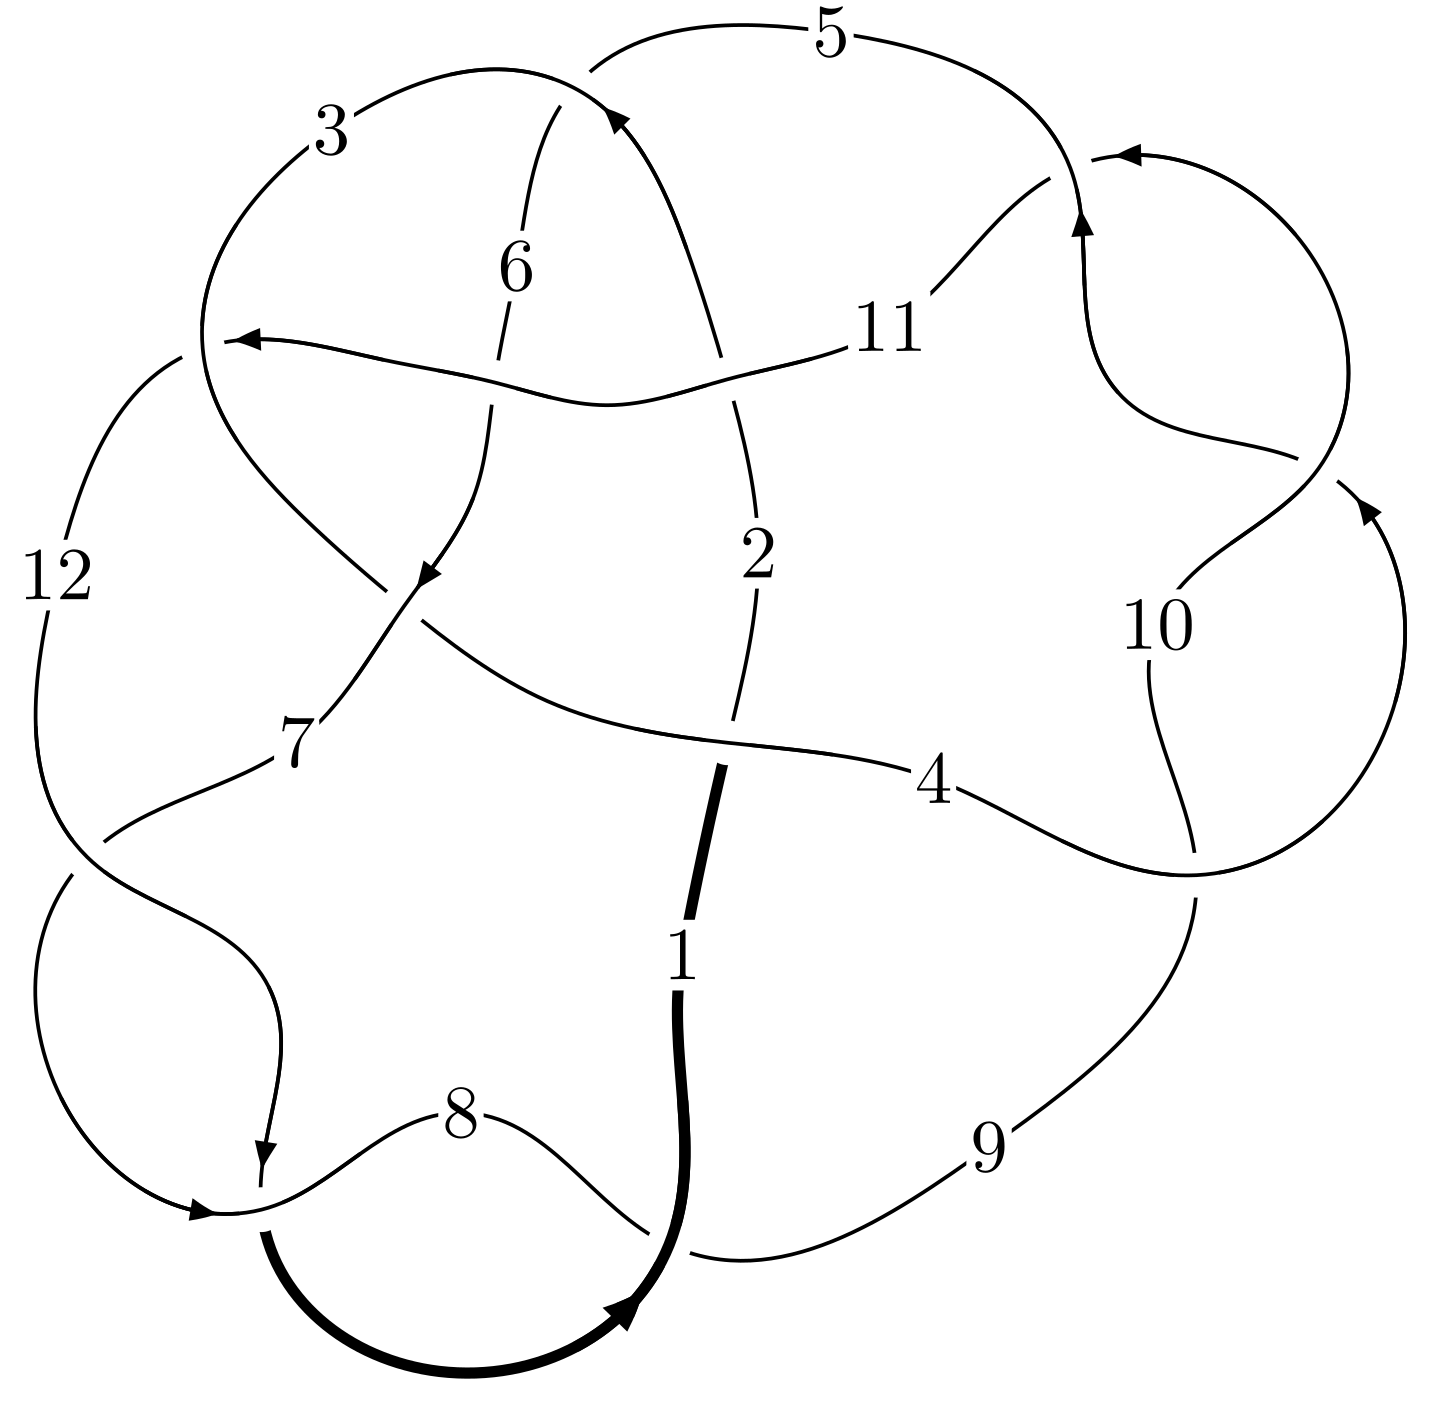
\includegraphics[width=112pt]{../../../GIT/diagram.site/Diagrams/png/2797_12n_0708.png}\\
\ \ \ A knot diagram\footnotemark}&
\allowdisplaybreaks
\textbf{Linearized knot diagam} \\
\cline{2-2}
 &
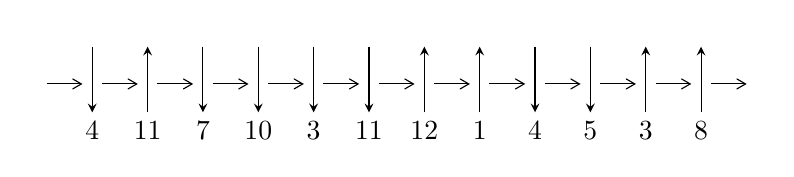
\begin{tikzpicture}[x=20pt, y=17pt]
	% nodes
	\node (C0) at (0, 0) {};
	\node (C1) at (1, 0) {};
	\node (C1U) at (1, +1) {};
	\node (C1D) at (1, -1) {4};

	\node (C2) at (2, 0) {};
	\node (C2U) at (2, +1) {};
	\node (C2D) at (2, -1) {11};

	\node (C3) at (3, 0) {};
	\node (C3U) at (3, +1) {};
	\node (C3D) at (3, -1) {7};

	\node (C4) at (4, 0) {};
	\node (C4U) at (4, +1) {};
	\node (C4D) at (4, -1) {10};

	\node (C5) at (5, 0) {};
	\node (C5U) at (5, +1) {};
	\node (C5D) at (5, -1) {3};

	\node (C6) at (6, 0) {};
	\node (C6U) at (6, +1) {};
	\node (C6D) at (6, -1) {11};

	\node (C7) at (7, 0) {};
	\node (C7U) at (7, +1) {};
	\node (C7D) at (7, -1) {12};

	\node (C8) at (8, 0) {};
	\node (C8U) at (8, +1) {};
	\node (C8D) at (8, -1) {1};

	\node (C9) at (9, 0) {};
	\node (C9U) at (9, +1) {};
	\node (C9D) at (9, -1) {4};

	\node (C10) at (10, 0) {};
	\node (C10U) at (10, +1) {};
	\node (C10D) at (10, -1) {5};

	\node (C11) at (11, 0) {};
	\node (C11U) at (11, +1) {};
	\node (C11D) at (11, -1) {3};

	\node (C12) at (12, 0) {};
	\node (C12U) at (12, +1) {};
	\node (C12D) at (12, -1) {8};
	\node (C13) at (13, 0) {};

	% arrows
	\draw[->,>={angle 60}]
	(C0) edge (C1) (C1) edge (C2) (C2) edge (C3) (C3) edge (C4) (C4) edge (C5) (C5) edge (C6) (C6) edge (C7) (C7) edge (C8) (C8) edge (C9) (C9) edge (C10) (C10) edge (C11) (C11) edge (C12) (C12) edge (C13) ;	\draw[->,>=stealth]
	(C1U) edge (C1D) (C2D) edge (C2U) (C3U) edge (C3D) (C4U) edge (C4D) (C5U) edge (C5D) (C6U) edge (C6D) (C7D) edge (C7U) (C8D) edge (C8U) (C9U) edge (C9D) (C10U) edge (C10D) (C11D) edge (C11U) (C12D) edge (C12U) ;
	\end{tikzpicture} \\
\hhline{~~} \\& 
\textbf{Solving Sequence} \\ \cline{2-2} 
 &
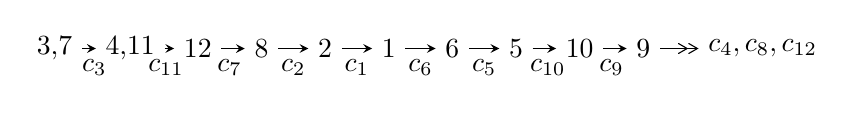
\begin{tikzpicture}[x=23pt, y=7pt]
	% node
	\node (A0) at (-1/8, 0) {3,7};
	\node (A1) at (17/16, 0) {4,11};
	\node (A2) at (17/8, 0) {12};
	\node (A3) at (25/8, 0) {8};
	\node (A4) at (33/8, 0) {2};
	\node (A5) at (41/8, 0) {1};
	\node (A6) at (49/8, 0) {6};
	\node (A7) at (57/8, 0) {5};
	\node (A8) at (65/8, 0) {10};
	\node (A9) at (73/8, 0) {9};
	\node (C1) at (1/2, -1) {$c_{3}$};
	\node (C2) at (13/8, -1) {$c_{11}$};
	\node (C3) at (21/8, -1) {$c_{7}$};
	\node (C4) at (29/8, -1) {$c_{2}$};
	\node (C5) at (37/8, -1) {$c_{1}$};
	\node (C6) at (45/8, -1) {$c_{6}$};
	\node (C7) at (53/8, -1) {$c_{5}$};
	\node (C8) at (61/8, -1) {$c_{10}$};
	\node (C9) at (69/8, -1) {$c_{9}$};
	\node (A10) at (11, 0) {$c_{4},c_{8},c_{12}$};

	% edge
	\draw[->,>=stealth]	
	(A0) edge (A1) (A1) edge (A2) (A2) edge (A3) (A3) edge (A4) (A4) edge (A5) (A5) edge (A6) (A6) edge (A7) (A7) edge (A8) (A8) edge (A9) ;
	\draw[->>,>={angle 60}]	
	(A9) edge (A10);
\end{tikzpicture} \\ 

\end{tabular} \\

\footnotetext{
The image of knot diagram is generated by the software ``\textbf{Draw programme}" developed by Andrew Bartholomew(\url{http://www.layer8.co.uk/maths/draw/index.htm\#Running-draw}), where we modified some parts for our purpose(\url{https://github.com/CATsTAILs/LinksPainter}).
}\phantom \\ \newline 
\centering \textbf{Ideals for irreducible components\footnotemark of $X_{\text{par}}$} 
 
\begin{align*}
I^u_{1}&=\langle 
1.10576\times10^{47} u^{33}-8.01097\times10^{47} u^{32}+\cdots+1.80128\times10^{49} b+1.32887\times10^{49},\\
\phantom{I^u_{1}}&\phantom{= \langle  }-1.30799\times10^{49} u^{33}+3.04903\times10^{49} u^{32}+\cdots+8.46601\times10^{50} a+1.20480\times10^{51},\\
\phantom{I^u_{1}}&\phantom{= \langle  }u^{34}-3 u^{33}+\cdots+119 u-47\rangle \\
I^u_{2}&=\langle 
u^8+2 u^7- u^6-2 u^5+u^4+b-1,\;- u^8-2 u^7+u^6+2 u^5- u^4- u^3- u^2+a+u+1,\\
\phantom{I^u_{2}}&\phantom{= \langle  }u^{10}+2 u^9- u^8- u^7+2 u^6- u^5+u^4-2 u^2+u-1\rangle \\
\\
\end{align*}
\raggedright * 2 irreducible components of $\dim_{\mathbb{C}}=0$, with total 44 representations.\\
\footnotetext{All coefficients of polynomials are rational numbers. But the coefficients are sometimes approximated in decimal forms when there is not enough margin.}
\newpage
\renewcommand{\arraystretch}{1}
\centering \section*{I. $I^u_{1}= \langle 1.11\times10^{47} u^{33}-8.01\times10^{47} u^{32}+\cdots+1.80\times10^{49} b+1.33\times10^{49},\;-1.31\times10^{49} u^{33}+3.05\times10^{49} u^{32}+\cdots+8.47\times10^{50} a+1.20\times10^{51},\;u^{34}-3 u^{33}+\cdots+119 u-47 \rangle$}
\flushleft \textbf{(i) Arc colorings}\\
\begin{tabular}{m{7pt} m{180pt} m{7pt} m{180pt} }
\flushright $a_{3}=$&$\begin{pmatrix}1\\0\end{pmatrix}$ \\
\flushright $a_{7}=$&$\begin{pmatrix}0\\u\end{pmatrix}$ \\
\flushright $a_{4}=$&$\begin{pmatrix}1\\u^2\end{pmatrix}$ \\
\flushright $a_{11}=$&$\begin{pmatrix}0.0154499 u^{33}-0.0360149 u^{32}+\cdots+0.941098 u-1.42310\\-0.00613876 u^{33}+0.0444738 u^{32}+\cdots+2.98012 u-0.737735\end{pmatrix}$ \\
\flushright $a_{12}=$&$\begin{pmatrix}0.00931114 u^{33}+0.00845885 u^{32}+\cdots+3.92122 u-2.16083\\-0.00613876 u^{33}+0.0444738 u^{32}+\cdots+2.98012 u-0.737735\end{pmatrix}$ \\
\flushright $a_{8}=$&$\begin{pmatrix}0.00533206 u^{33}-0.0235388 u^{32}+\cdots-3.14642 u+1.53400\\0.0239032 u^{33}-0.0742285 u^{32}+\cdots-2.18646 u+0.793400\end{pmatrix}$ \\
\flushright $a_{2}=$&$\begin{pmatrix}0.0232060 u^{33}-0.0633719 u^{32}+\cdots-1.53624 u+0.592137\\-0.00632519 u^{33}+0.0366325 u^{32}+\cdots+3.07109 u-0.769781\end{pmatrix}$ \\
\flushright $a_{1}=$&$\begin{pmatrix}0.0236972 u^{33}-0.0414540 u^{32}+\cdots+1.18747 u-0.471217\\-0.000941418 u^{33}-0.00268565 u^{32}+\cdots+0.310591 u+0.329618\end{pmatrix}$ \\
\flushright $a_{6}=$&$\begin{pmatrix}-0.0248174 u^{33}+0.0762449 u^{32}+\cdots+3.20943 u-0.350085\\0.00624624 u^{33}-0.0255551 u^{32}+\cdots-2.16938 u+1.09068\end{pmatrix}$ \\
\flushright $a_{5}=$&$\begin{pmatrix}-0.0185712 u^{33}+0.0506897 u^{32}+\cdots+1.04004 u+0.740599\\0.00624624 u^{33}-0.0255551 u^{32}+\cdots-2.16938 u+1.09068\end{pmatrix}$ \\
\flushright $a_{10}=$&$\begin{pmatrix}0.0156673 u^{33}-0.0416737 u^{32}+\cdots+3.51356 u-2.20491\\-0.0217802 u^{33}+0.0517956 u^{32}+\cdots-0.173101 u+1.00253\end{pmatrix}$ \\
\flushright $a_{9}=$&$\begin{pmatrix}0.0250751 u^{33}-0.0635130 u^{32}+\cdots+3.23816 u-1.45281\\-0.0328754 u^{33}+0.0519114 u^{32}+\cdots-0.490626 u+1.30257\end{pmatrix}$\\&\end{tabular}
\flushleft \textbf{(ii) Obstruction class $= -1$}\\~\\
\flushleft \textbf{(iii) Cusp Shapes $= -0.338570 u^{33}+0.808896 u^{32}+\cdots+19.1088 u+0.740160$}\\~\\
\newpage\renewcommand{\arraystretch}{1}
\flushleft \textbf{(iv) u-Polynomials at the component}\newline \\
\begin{tabular}{m{50pt}|m{274pt}}
Crossings & \hspace{64pt}u-Polynomials at each crossing \\
\hline $$\begin{aligned}c_{1}\end{aligned}$$&$\begin{aligned}
&u^{34}-4 u^{33}+\cdots+612 u-536
\end{aligned}$\\
\hline $$\begin{aligned}c_{2},c_{11}\end{aligned}$$&$\begin{aligned}
&u^{34}-2 u^{33}+\cdots+22 u+1
\end{aligned}$\\
\hline $$\begin{aligned}c_{3}\end{aligned}$$&$\begin{aligned}
&u^{34}+3 u^{33}+\cdots-119 u-47
\end{aligned}$\\
\hline $$\begin{aligned}c_{4},c_{9},c_{10}\end{aligned}$$&$\begin{aligned}
&u^{34}+u^{33}+\cdots-3 u-1
\end{aligned}$\\
\hline $$\begin{aligned}c_{5}\end{aligned}$$&$\begin{aligned}
&u^{34}-2 u^{33}+\cdots-30 u+25
\end{aligned}$\\
\hline $$\begin{aligned}c_{6}\end{aligned}$$&$\begin{aligned}
&u^{34}- u^{33}+\cdots-80 u-8
\end{aligned}$\\
\hline $$\begin{aligned}c_{7},c_{8},c_{12}\end{aligned}$$&$\begin{aligned}
&u^{34}+2 u^{33}+\cdots-11 u-1
\end{aligned}$\\
\hline
\end{tabular}\\~\\
\newpage\renewcommand{\arraystretch}{1}
\flushleft \textbf{(v) Riley Polynomials at the component}\newline \\
\begin{tabular}{m{50pt}|m{274pt}}
Crossings & \hspace{64pt}Riley Polynomials at each crossing \\
\hline $$\begin{aligned}c_{1}\end{aligned}$$&$\begin{aligned}
&y^{34}+52 y^{33}+\cdots+3454640 y+287296
\end{aligned}$\\
\hline $$\begin{aligned}c_{2},c_{11}\end{aligned}$$&$\begin{aligned}
&y^{34}-40 y^{33}+\cdots-426 y+1
\end{aligned}$\\
\hline $$\begin{aligned}c_{3}\end{aligned}$$&$\begin{aligned}
&y^{34}+7 y^{33}+\cdots+23815 y+2209
\end{aligned}$\\
\hline $$\begin{aligned}c_{4},c_{9},c_{10}\end{aligned}$$&$\begin{aligned}
&y^{34}-23 y^{33}+\cdots-9 y+1
\end{aligned}$\\
\hline $$\begin{aligned}c_{5}\end{aligned}$$&$\begin{aligned}
&y^{34}+44 y^{33}+\cdots-27550 y+625
\end{aligned}$\\
\hline $$\begin{aligned}c_{6}\end{aligned}$$&$\begin{aligned}
&y^{34}+53 y^{33}+\cdots-6560 y+64
\end{aligned}$\\
\hline $$\begin{aligned}c_{7},c_{8},c_{12}\end{aligned}$$&$\begin{aligned}
&y^{34}-44 y^{33}+\cdots-261 y+1
\end{aligned}$\\
\hline
\end{tabular}\\~\\
\newpage\flushleft \textbf{(vi) Complex Volumes and Cusp Shapes}
$$\begin{array}{c|c|c}  
\text{Solutions to }I^u_{1}& \I (\text{vol} + \sqrt{-1}CS) & \text{Cusp shape}\\
 \hline 
\begin{aligned}
u &= \phantom{-}0.469797 + 0.926681 I \\
a &= \phantom{-}0.173533 + 0.105962 I \\
b &= -0.73202 + 1.30784 I\end{aligned}
 & \phantom{-}6.31099 - 6.15435 I & \phantom{-}0.40584 + 7.42268 I \\ \hline\begin{aligned}
u &= \phantom{-}0.469797 - 0.926681 I \\
a &= \phantom{-}0.173533 - 0.105962 I \\
b &= -0.73202 - 1.30784 I\end{aligned}
 & \phantom{-}6.31099 + 6.15435 I & \phantom{-}0.40584 - 7.42268 I \\ \hline\begin{aligned}
u &= \phantom{-}0.055016 + 0.907256 I \\
a &= -2.57529 + 0.34754 I \\
b &= \phantom{-}1.334640 - 0.108463 I\end{aligned}
 & \phantom{-}2.75863 - 1.86345 I & \phantom{-}3.58957 + 3.82529 I \\ \hline\begin{aligned}
u &= \phantom{-}0.055016 - 0.907256 I \\
a &= -2.57529 - 0.34754 I \\
b &= \phantom{-}1.334640 + 0.108463 I\end{aligned}
 & \phantom{-}2.75863 + 1.86345 I & \phantom{-}3.58957 - 3.82529 I \\ \hline\begin{aligned}
u &= -0.597332 + 0.940180 I \\
a &= \phantom{-}0.729498 - 0.532364 I \\
b &= -1.41321 - 0.68276 I\end{aligned}
 & \phantom{-}8.66900 + 2.33850 I & \phantom{-}4.06570 - 4.09223 I \\ \hline\begin{aligned}
u &= -0.597332 - 0.940180 I \\
a &= \phantom{-}0.729498 + 0.532364 I \\
b &= -1.41321 + 0.68276 I\end{aligned}
 & \phantom{-}8.66900 - 2.33850 I & \phantom{-}4.06570 + 4.09223 I \\ \hline\begin{aligned}
u &= \phantom{-}0.548448 + 0.661548 I \\
a &= -0.395572 + 0.002411 I \\
b &= \phantom{-}0.361280 - 0.917030 I\end{aligned}
 & -0.97085 - 3.73329 I & -3.26740 + 7.90292 I \\ \hline\begin{aligned}
u &= \phantom{-}0.548448 - 0.661548 I \\
a &= -0.395572 - 0.002411 I \\
b &= \phantom{-}0.361280 + 0.917030 I\end{aligned}
 & -0.97085 + 3.73329 I & -3.26740 - 7.90292 I \\ \hline\begin{aligned}
u &= -0.838637\phantom{ +0.000000I} \\
a &= -1.95743\phantom{ +0.000000I} \\
b &= \phantom{-}0.627035\phantom{ +0.000000I}\end{aligned}
 & -4.25399\phantom{ +0.000000I} & \phantom{-}2.99560\phantom{ +0.000000I} \\ \hline\begin{aligned}
u &= \phantom{-}0.526405 + 1.043420 I \\
a &= -0.384792 + 1.231010 I \\
b &= -0.333049 + 0.008900 I\end{aligned}
 & \phantom{-}6.57922 + 1.93235 I & \phantom{-}0.558019 - 0.700654 I\\
 \hline 
 \end{array}$$\newpage$$\begin{array}{c|c|c}  
\text{Solutions to }I^u_{1}& \I (\text{vol} + \sqrt{-1}CS) & \text{Cusp shape}\\
 \hline 
\begin{aligned}
u &= \phantom{-}0.526405 - 1.043420 I \\
a &= -0.384792 - 1.231010 I \\
b &= -0.333049 - 0.008900 I\end{aligned}
 & \phantom{-}6.57922 - 1.93235 I & \phantom{-}0.558019 + 0.700654 I \\ \hline\begin{aligned}
u &= -0.572947 + 1.025320 I \\
a &= \phantom{-}0.483665 - 1.056480 I \\
b &= -1.052410 - 0.236751 I\end{aligned}
 & \phantom{-}8.94084 + 2.54032 I & \phantom{-}3.06411 - 2.90404 I \\ \hline\begin{aligned}
u &= -0.572947 - 1.025320 I \\
a &= \phantom{-}0.483665 + 1.056480 I \\
b &= -1.052410 + 0.236751 I\end{aligned}
 & \phantom{-}8.94084 - 2.54032 I & \phantom{-}3.06411 + 2.90404 I \\ \hline\begin{aligned}
u &= \phantom{-}0.001919 + 0.788798 I \\
a &= -1.54872 + 0.07110 I \\
b &= \phantom{-}1.52564 + 0.31114 I\end{aligned}
 & \phantom{-}2.45487 + 1.58321 I & \phantom{-}5.81072 - 4.19715 I \\ \hline\begin{aligned}
u &= \phantom{-}0.001919 - 0.788798 I \\
a &= -1.54872 - 0.07110 I \\
b &= \phantom{-}1.52564 - 0.31114 I\end{aligned}
 & \phantom{-}2.45487 - 1.58321 I & \phantom{-}5.81072 + 4.19715 I \\ \hline\begin{aligned}
u &= \phantom{-}0.758673\phantom{ +0.000000I} \\
a &= \phantom{-}0.528592\phantom{ +0.000000I} \\
b &= -0.0495765\phantom{ +0.000000I}\end{aligned}
 & -0.995684\phantom{ +0.000000I} & -12.7630\phantom{ +0.000000I} \\ \hline\begin{aligned}
u &= \phantom{-}0.603373 + 0.439110 I \\
a &= \phantom{-}0.858658 - 0.248549 I \\
b &= \phantom{-}0.056009 + 0.383780 I\end{aligned}
 & -1.379030 - 0.087279 I & -5.81206 - 0.48445 I \\ \hline\begin{aligned}
u &= \phantom{-}0.603373 - 0.439110 I \\
a &= \phantom{-}0.858658 + 0.248549 I \\
b &= \phantom{-}0.056009 - 0.383780 I\end{aligned}
 & -1.379030 + 0.087279 I & -5.81206 + 0.48445 I \\ \hline\begin{aligned}
u &= -0.716829 + 1.057590 I \\
a &= \phantom{-}1.24846 - 0.72721 I \\
b &= -1.51816 - 0.17886 I\end{aligned}
 & \phantom{-}8.00595 + 3.00523 I & \phantom{-}3.73808 - 2.90092 I \\ \hline\begin{aligned}
u &= -0.716829 - 1.057590 I \\
a &= \phantom{-}1.24846 + 0.72721 I \\
b &= -1.51816 + 0.17886 I\end{aligned}
 & \phantom{-}8.00595 - 3.00523 I & \phantom{-}3.73808 + 2.90092 I\\
 \hline 
 \end{array}$$\newpage$$\begin{array}{c|c|c}  
\text{Solutions to }I^u_{1}& \I (\text{vol} + \sqrt{-1}CS) & \text{Cusp shape}\\
 \hline 
\begin{aligned}
u &= \phantom{-}0.691711 + 1.120790 I \\
a &= \phantom{-}1.60001 + 0.60370 I \\
b &= -1.48377 + 0.32078 I\end{aligned}
 & \phantom{-}5.01121 - 8.11532 I & \phantom{-}0.18101 + 6.85241 I \\ \hline\begin{aligned}
u &= \phantom{-}0.691711 - 1.120790 I \\
a &= \phantom{-}1.60001 - 0.60370 I \\
b &= -1.48377 - 0.32078 I\end{aligned}
 & \phantom{-}5.01121 + 8.11532 I & \phantom{-}0.18101 - 6.85241 I \\ \hline\begin{aligned}
u &= \phantom{-}0.881012 + 0.992412 I \\
a &= \phantom{-}1.080060 + 0.559009 I \\
b &= -1.51362 - 0.11800 I\end{aligned}
 & \phantom{-}4.18213 + 1.75454 I & \phantom{-}1.44552 - 1.15085 I \\ \hline\begin{aligned}
u &= \phantom{-}0.881012 - 0.992412 I \\
a &= \phantom{-}1.080060 - 0.559009 I \\
b &= -1.51362 + 0.11800 I\end{aligned}
 & \phantom{-}4.18213 - 1.75454 I & \phantom{-}1.44552 + 1.15085 I \\ \hline\begin{aligned}
u &= -0.202533 + 0.473694 I \\
a &= -0.566502 + 0.966055 I \\
b &= \phantom{-}0.571429 + 0.385434 I\end{aligned}
 & \phantom{-}1.190200 + 0.722922 I & \phantom{-}4.39709 - 2.39918 I \\ \hline\begin{aligned}
u &= -0.202533 - 0.473694 I \\
a &= -0.566502 - 0.966055 I \\
b &= \phantom{-}0.571429 - 0.385434 I\end{aligned}
 & \phantom{-}1.190200 - 0.722922 I & \phantom{-}4.39709 + 2.39918 I \\ \hline\begin{aligned}
u &= -1.48547\phantom{ +0.000000I} \\
a &= \phantom{-}0.692495\phantom{ +0.000000I} \\
b &= -0.738006\phantom{ +0.000000I}\end{aligned}
 & -7.70081\phantom{ +0.000000I} & -22.1680\phantom{ +0.000000I} \\ \hline\begin{aligned}
u &= -1.49245\phantom{ +0.000000I} \\
a &= -0.0553962\phantom{ +0.000000I} \\
b &= \phantom{-}0.874161\phantom{ +0.000000I}\end{aligned}
 & -3.40883\phantom{ +0.000000I} & -1.08290\phantom{ +0.000000I} \\ \hline\begin{aligned}
u &= \phantom{-}1.13577 + 1.43590 I \\
a &= -1.174670 - 0.437080 I \\
b &= \phantom{-}1.65946 - 0.37041 I\end{aligned}
 & \phantom{-}14.0582 - 11.9947 I & \phantom{-0.000000 } 0 \\ \hline\begin{aligned}
u &= \phantom{-}1.13577 - 1.43590 I \\
a &= -1.174670 + 0.437080 I \\
b &= \phantom{-}1.65946 + 0.37041 I\end{aligned}
 & \phantom{-}14.0582 + 11.9947 I & \phantom{-0.000000 } 0\\
 \hline 
 \end{array}$$\newpage$$\begin{array}{c|c|c}  
\text{Solutions to }I^u_{1}& \I (\text{vol} + \sqrt{-1}CS) & \text{Cusp shape}\\
 \hline 
\begin{aligned}
u &= -1.29108 + 1.38239 I \\
a &= -1.068980 + 0.541449 I \\
b &= \phantom{-}1.65562 + 0.16606 I\end{aligned}
 & \phantom{-}18.1169 + 4.9950 I & \phantom{-0.000000 } 0 \\ \hline\begin{aligned}
u &= -1.29108 - 1.38239 I \\
a &= -1.068980 - 0.541449 I \\
b &= \phantom{-}1.65562 - 0.16606 I\end{aligned}
 & \phantom{-}18.1169 - 4.9950 I & \phantom{-0.000000 } 0 \\ \hline\begin{aligned}
u &= \phantom{-}1.49621 + 1.30271 I \\
a &= -0.882637 - 0.559769 I \\
b &= \phantom{-}1.52536 + 0.01034 I\end{aligned}
 & \phantom{-}13.07780 + 1.99862 I & \phantom{-0.000000 } 0 \\ \hline\begin{aligned}
u &= \phantom{-}1.49621 - 1.30271 I \\
a &= -0.882637 + 0.559769 I \\
b &= \phantom{-}1.52536 - 0.01034 I\end{aligned}
 & \phantom{-}13.07780 - 1.99862 I & \phantom{-0.000000 } 0\\
 \hline 
 \end{array}$$\newpage\newpage\renewcommand{\arraystretch}{1}
\centering \section*{II. $I^u_{2}= \langle u^8+2 u^7- u^6-2 u^5+u^4+b-1,\;- u^8-2 u^7+\cdots+a+1,\;u^{10}+2 u^9+\cdots+u-1 \rangle$}
\flushleft \textbf{(i) Arc colorings}\\
\begin{tabular}{m{7pt} m{180pt} m{7pt} m{180pt} }
\flushright $a_{3}=$&$\begin{pmatrix}1\\0\end{pmatrix}$ \\
\flushright $a_{7}=$&$\begin{pmatrix}0\\u\end{pmatrix}$ \\
\flushright $a_{4}=$&$\begin{pmatrix}1\\u^2\end{pmatrix}$ \\
\flushright $a_{11}=$&$\begin{pmatrix}u^8+2 u^7- u^6-2 u^5+u^4+u^3+u^2- u-1\\- u^8-2 u^7+u^6+2 u^5- u^4+1\end{pmatrix}$ \\
\flushright $a_{12}=$&$\begin{pmatrix}u^3+u^2- u\\- u^8-2 u^7+u^6+2 u^5- u^4+1\end{pmatrix}$ \\
\flushright $a_{8}=$&$\begin{pmatrix}u^7+2 u^6- u^5-2 u^4+u^3\\u^9+2 u^8- u^7- u^6+2 u^5-2 u^4+u^2- u+1\end{pmatrix}$ \\
\flushright $a_{2}=$&$\begin{pmatrix}u^9+3 u^8+u^7-2 u^6+u^5+u^4+u^2-2 u-1\\- u^3- u^2+u+1\end{pmatrix}$ \\
\flushright $a_{1}=$&$\begin{pmatrix}u^9+3 u^8+u^7-2 u^6+u^5+u^4- u^3- u-1\\- u^5- u^4- u^2+u+1\end{pmatrix}$ \\
\flushright $a_{6}=$&$\begin{pmatrix}-2 u^9-4 u^8+3 u^7+4 u^6-5 u^5+u^4- u^2+5 u-2\\u^9+2 u^8- u^7- u^6+2 u^5- u^4+u^3-2 u+1\end{pmatrix}$ \\
\flushright $a_{5}=$&$\begin{pmatrix}- u^9-2 u^8+2 u^7+3 u^6-3 u^5+u^3- u^2+3 u-1\\u^9+2 u^8- u^7- u^6+2 u^5- u^4+u^3-2 u+1\end{pmatrix}$ \\
\flushright $a_{10}=$&$\begin{pmatrix}u^7+u^6-2 u^5+u^3+2 u-2\\u^9+u^8-3 u^7- u^6+3 u^5+u^3- u^2- u+1\end{pmatrix}$ \\
\flushright $a_{9}=$&$\begin{pmatrix}u^2+u-1\\- u^7- u^6+2 u^5+u^4- u+1\end{pmatrix}$\\&\end{tabular}
\flushleft \textbf{(ii) Obstruction class $= 1$}\\~\\
\flushleft \textbf{(iii) Cusp Shapes $= 2 u^9+4 u^8+3 u^7+4 u^6-4 u^5- u^4+7 u^3-3 u^2+2 u-4$}\\~\\
\newpage\renewcommand{\arraystretch}{1}
\flushleft \textbf{(iv) u-Polynomials at the component}\newline \\
\begin{tabular}{m{50pt}|m{274pt}}
Crossings & \hspace{64pt}u-Polynomials at each crossing \\
\hline $$\begin{aligned}c_{1}\end{aligned}$$&$\begin{aligned}
&u^{10}+3 u^9+6 u^8+6 u^7+u^6-11 u^5-14 u^4- u^3+8 u^2+3 u-1
\end{aligned}$\\
\hline $$\begin{aligned}c_{2}\end{aligned}$$&$\begin{aligned}
&u^{10}+3 u^9-2 u^8-14 u^7-5 u^6+23 u^5+16 u^4-15 u^3-11 u^2+4 u+1
\end{aligned}$\\
\hline $$\begin{aligned}c_{3}\end{aligned}$$&$\begin{aligned}
&u^{10}+2 u^9- u^8- u^7+2 u^6- u^5+u^4-2 u^2+u-1
\end{aligned}$\\
\hline $$\begin{aligned}c_{4}\end{aligned}$$&$\begin{aligned}
&u^{10}-6 u^8- u^7+13 u^6+4 u^5-13 u^4-5 u^3+6 u^2+3 u-1
\end{aligned}$\\
\hline $$\begin{aligned}c_{5}\end{aligned}$$&$\begin{aligned}
&u^{10}+u^9+2 u^8- u^6- u^5-2 u^4- u^3+u^2+2 u-1
\end{aligned}$\\
\hline $$\begin{aligned}c_{6}\end{aligned}$$&$\begin{aligned}
&u^{10}+2 u^8-2 u^7- u^6-4 u^5-2 u^4+3 u^3-2 u^2+3 u+1
\end{aligned}$\\
\hline $$\begin{aligned}c_{7},c_{8}\end{aligned}$$&$\begin{aligned}
&u^{10}+u^9-6 u^8-6 u^7+11 u^6+11 u^5-4 u^4-5 u^3-4 u^2- u+1
\end{aligned}$\\
\hline $$\begin{aligned}c_{9},c_{10}\end{aligned}$$&$\begin{aligned}
&u^{10}-6 u^8+u^7+13 u^6-4 u^5-13 u^4+5 u^3+6 u^2-3 u-1
\end{aligned}$\\
\hline $$\begin{aligned}c_{11}\end{aligned}$$&$\begin{aligned}
&u^{10}-3 u^9-2 u^8+14 u^7-5 u^6-23 u^5+16 u^4+15 u^3-11 u^2-4 u+1
\end{aligned}$\\
\hline $$\begin{aligned}c_{12}\end{aligned}$$&$\begin{aligned}
&u^{10}- u^9-6 u^8+6 u^7+11 u^6-11 u^5-4 u^4+5 u^3-4 u^2+u+1
\end{aligned}$\\
\hline
\end{tabular}\\~\\
\newpage\renewcommand{\arraystretch}{1}
\flushleft \textbf{(v) Riley Polynomials at the component}\newline \\
\begin{tabular}{m{50pt}|m{274pt}}
Crossings & \hspace{64pt}Riley Polynomials at each crossing \\
\hline $$\begin{aligned}c_{1}\end{aligned}$$&$\begin{aligned}
&y^{10}+3 y^9+\cdots-25 y+1
\end{aligned}$\\
\hline $$\begin{aligned}c_{2},c_{11}\end{aligned}$$&$\begin{aligned}
&y^{10}-13 y^9+\cdots-38 y+1
\end{aligned}$\\
\hline $$\begin{aligned}c_{3}\end{aligned}$$&$\begin{aligned}
&y^{10}-6 y^9+9 y^8+y^7-4 y^6+y^5-3 y^4-6 y^3+2 y^2+3 y+1
\end{aligned}$\\
\hline $$\begin{aligned}c_{4},c_{9},c_{10}\end{aligned}$$&$\begin{aligned}
&y^{10}-12 y^9+\cdots-21 y+1
\end{aligned}$\\
\hline $$\begin{aligned}c_{5}\end{aligned}$$&$\begin{aligned}
&y^{10}+3 y^9+2 y^8-6 y^7-3 y^6+y^5-4 y^4+y^3+9 y^2-6 y+1
\end{aligned}$\\
\hline $$\begin{aligned}c_{6}\end{aligned}$$&$\begin{aligned}
&y^{10}+4 y^9+2 y^8-12 y^7-27 y^6-6 y^5+48 y^4+21 y^3-18 y^2-13 y+1
\end{aligned}$\\
\hline $$\begin{aligned}c_{7},c_{8},c_{12}\end{aligned}$$&$\begin{aligned}
&y^{10}-13 y^9+\cdots-9 y+1
\end{aligned}$\\
\hline
\end{tabular}\\~\\
\newpage\flushleft \textbf{(vi) Complex Volumes and Cusp Shapes}
$$\begin{array}{c|c|c}  
\text{Solutions to }I^u_{2}& \I (\text{vol} + \sqrt{-1}CS) & \text{Cusp shape}\\
 \hline 
\begin{aligned}
u &= \phantom{-}0.748756 + 0.648482 I \\
a &= \phantom{-}0.375274 + 0.762613 I \\
b &= -1.50876 + 0.37799 I\end{aligned}
 & \phantom{-}8.36725 - 1.33489 I & \phantom{-}1.94242 - 2.46421 I \\ \hline\begin{aligned}
u &= \phantom{-}0.748756 - 0.648482 I \\
a &= \phantom{-}0.375274 - 0.762613 I \\
b &= -1.50876 - 0.37799 I\end{aligned}
 & \phantom{-}8.36725 + 1.33489 I & \phantom{-}1.94242 + 2.46421 I \\ \hline\begin{aligned}
u &= \phantom{-}0.937843\phantom{ +0.000000I} \\
a &= \phantom{-}0.283456\phantom{ +0.000000I} \\
b &= \phantom{-}0.483130\phantom{ +0.000000I}\end{aligned}
 & -0.498447\phantom{ +0.000000I} & \phantom{-}5.48800\phantom{ +0.000000I} \\ \hline\begin{aligned}
u &= -0.186579 + 0.862945 I \\
a &= \phantom{-}1.14726 - 1.04811 I \\
b &= -1.26022 - 0.68934 I\end{aligned}
 & \phantom{-}6.77164 + 4.55155 I & \phantom{-}1.99946 - 3.34420 I \\ \hline\begin{aligned}
u &= -0.186579 - 0.862945 I \\
a &= \phantom{-}1.14726 + 1.04811 I \\
b &= -1.26022 + 0.68934 I\end{aligned}
 & \phantom{-}6.77164 - 4.55155 I & \phantom{-}1.99946 + 3.34420 I \\ \hline\begin{aligned}
u &= -1.12602\phantom{ +0.000000I} \\
a &= \phantom{-}1.14998\phantom{ +0.000000I} \\
b &= -0.183747\phantom{ +0.000000I}\end{aligned}
 & -5.01118\phantom{ +0.000000I} & -8.63130\phantom{ +0.000000I} \\ \hline\begin{aligned}
u &= \phantom{-}0.213691 + 0.628245 I \\
a &= -2.16352 - 0.71377 I \\
b &= \phantom{-}1.357540 + 0.192129 I\end{aligned}
 & \phantom{-}1.63959 + 1.30650 I & -4.90826 - 0.15548 I \\ \hline\begin{aligned}
u &= \phantom{-}0.213691 - 0.628245 I \\
a &= -2.16352 + 0.71377 I \\
b &= \phantom{-}1.357540 - 0.192129 I\end{aligned}
 & \phantom{-}1.63959 - 1.30650 I & -4.90826 + 0.15548 I \\ \hline\begin{aligned}
u &= -1.55268\phantom{ +0.000000I} \\
a &= -0.662730\phantom{ +0.000000I} \\
b &= \phantom{-}0.883015\phantom{ +0.000000I}\end{aligned}
 & -7.45391\phantom{ +0.000000I} & \phantom{-}10.7450\phantom{ +0.000000I} \\ \hline\begin{aligned}
u &= -1.81088\phantom{ +0.000000I} \\
a &= \phantom{-}0.511259\phantom{ +0.000000I} \\
b &= -1.35950\phantom{ +0.000000I}\end{aligned}
 & -0.854207\phantom{ +0.000000I} & \phantom{-}1.33140\phantom{ +0.000000I}\\
 \hline 
 \end{array}$$\newpage
\newpage\renewcommand{\arraystretch}{1}
\centering \section*{ III. u-Polynomials}
\begin{tabular}{m{50pt}|m{274pt}}
Crossings & \hspace{64pt}u-Polynomials at each crossing \\
\hline $$\begin{aligned}c_{1}\end{aligned}$$&$\begin{aligned}
&(u^{10}+3 u^9+6 u^8+6 u^7+u^6-11 u^5-14 u^4- u^3+8 u^2+3 u-1)\\
&\cdot(u^{34}-4 u^{33}+\cdots+612 u-536)
\end{aligned}$\\
\hline $$\begin{aligned}c_{2}\end{aligned}$$&$\begin{aligned}
&(u^{10}+3 u^9-2 u^8-14 u^7-5 u^6+23 u^5+16 u^4-15 u^3-11 u^2+4 u+1)\\
&\cdot(u^{34}-2 u^{33}+\cdots+22 u+1)
\end{aligned}$\\
\hline $$\begin{aligned}c_{3}\end{aligned}$$&$\begin{aligned}
&(u^{10}+2 u^9- u^8- u^7+2 u^6- u^5+u^4-2 u^2+u-1)\\
&\cdot(u^{34}+3 u^{33}+\cdots-119 u-47)
\end{aligned}$\\
\hline $$\begin{aligned}c_{4}\end{aligned}$$&$\begin{aligned}
&(u^{10}-6 u^8- u^7+13 u^6+4 u^5-13 u^4-5 u^3+6 u^2+3 u-1)\\
&\cdot(u^{34}+u^{33}+\cdots-3 u-1)
\end{aligned}$\\
\hline $$\begin{aligned}c_{5}\end{aligned}$$&$\begin{aligned}
&(u^{10}+u^9+2 u^8- u^6- u^5-2 u^4- u^3+u^2+2 u-1)\\
&\cdot(u^{34}-2 u^{33}+\cdots-30 u+25)
\end{aligned}$\\
\hline $$\begin{aligned}c_{6}\end{aligned}$$&$\begin{aligned}
&(u^{10}+2 u^8-2 u^7- u^6-4 u^5-2 u^4+3 u^3-2 u^2+3 u+1)\\
&\cdot(u^{34}- u^{33}+\cdots-80 u-8)
\end{aligned}$\\
\hline $$\begin{aligned}c_{7},c_{8}\end{aligned}$$&$\begin{aligned}
&(u^{10}+u^9-6 u^8-6 u^7+11 u^6+11 u^5-4 u^4-5 u^3-4 u^2- u+1)\\
&\cdot(u^{34}+2 u^{33}+\cdots-11 u-1)
\end{aligned}$\\
\hline $$\begin{aligned}c_{9},c_{10}\end{aligned}$$&$\begin{aligned}
&(u^{10}-6 u^8+u^7+13 u^6-4 u^5-13 u^4+5 u^3+6 u^2-3 u-1)\\
&\cdot(u^{34}+u^{33}+\cdots-3 u-1)
\end{aligned}$\\
\hline $$\begin{aligned}c_{11}\end{aligned}$$&$\begin{aligned}
&(u^{10}-3 u^9-2 u^8+14 u^7-5 u^6-23 u^5+16 u^4+15 u^3-11 u^2-4 u+1)\\
&\cdot(u^{34}-2 u^{33}+\cdots+22 u+1)
\end{aligned}$\\
\hline $$\begin{aligned}c_{12}\end{aligned}$$&$\begin{aligned}
&(u^{10}- u^9-6 u^8+6 u^7+11 u^6-11 u^5-4 u^4+5 u^3-4 u^2+u+1)\\
&\cdot(u^{34}+2 u^{33}+\cdots-11 u-1)
\end{aligned}$\\
\hline
\end{tabular}\newpage\renewcommand{\arraystretch}{1}
\centering \section*{ IV. Riley Polynomials}
\begin{tabular}{m{50pt}|m{274pt}}
Crossings & \hspace{64pt}Riley Polynomials at each crossing \\
\hline $$\begin{aligned}c_{1}\end{aligned}$$&$\begin{aligned}
&(y^{10}+3 y^9+\cdots-25 y+1)(y^{34}+52 y^{33}+\cdots+3454640 y+287296)
\end{aligned}$\\
\hline $$\begin{aligned}c_{2},c_{11}\end{aligned}$$&$\begin{aligned}
&(y^{10}-13 y^9+\cdots-38 y+1)(y^{34}-40 y^{33}+\cdots-426 y+1)
\end{aligned}$\\
\hline $$\begin{aligned}c_{3}\end{aligned}$$&$\begin{aligned}
&(y^{10}-6 y^9+9 y^8+y^7-4 y^6+y^5-3 y^4-6 y^3+2 y^2+3 y+1)\\
&\cdot(y^{34}+7 y^{33}+\cdots+23815 y+2209)
\end{aligned}$\\
\hline $$\begin{aligned}c_{4},c_{9},c_{10}\end{aligned}$$&$\begin{aligned}
&(y^{10}-12 y^9+\cdots-21 y+1)(y^{34}-23 y^{33}+\cdots-9 y+1)
\end{aligned}$\\
\hline $$\begin{aligned}c_{5}\end{aligned}$$&$\begin{aligned}
&(y^{10}+3 y^9+2 y^8-6 y^7-3 y^6+y^5-4 y^4+y^3+9 y^2-6 y+1)\\
&\cdot(y^{34}+44 y^{33}+\cdots-27550 y+625)
\end{aligned}$\\
\hline $$\begin{aligned}c_{6}\end{aligned}$$&$\begin{aligned}
&(y^{10}+4 y^9+2 y^8-12 y^7-27 y^6-6 y^5+48 y^4+21 y^3-18 y^2-13 y+1)\\
&\cdot(y^{34}+53 y^{33}+\cdots-6560 y+64)
\end{aligned}$\\
\hline $$\begin{aligned}c_{7},c_{8},c_{12}\end{aligned}$$&$\begin{aligned}
&(y^{10}-13 y^9+\cdots-9 y+1)(y^{34}-44 y^{33}+\cdots-261 y+1)
\end{aligned}$\\
\hline
\end{tabular}
\vskip 2pc
\end{document}